\section{Ejercicio Resuelto}

A continuación resolvemos el problema de flujo resumido en la
Fig.~\ref{enu01}.  Se busca reproducir el flujo de agua en un suelo
isótropo que tiene un espesor de 9.2 metros, está formado por arena
limosa con coeficiente de permeabilidad ($k_x=k_y=k_z=5\cdot10^{-5}$
m/s) y limita en su parte inferior con una capa de arcilla
impermeable.  En este estrato arenoso se ha clavado 4.6 m de una
tablestaca que asumiremos de longitud infinita en la dirección
perpendicular al plano del dibujo. A la izquierda de la tablestaca
(aguasarriba) se ha acumulado una altura de 3 metros de agua y a la
derecha (aguas abajo) la escorrentía hace no haya acumulación de
agua. Para el problema así definido y asumiendo un régimen
estacionario se pide:
\begin{enumerate}
\item Obtener el flujo de agua saliente aguas abajo (por unidad de
  longitud de la dirección $y$).
\item Obtener la evolución de la carga total del fluido en el camino
  BCD y estimar el valor del gradiente hidraúlico en el punto D.
\end{enumerate}

\begin{figure}[!h]
  \begin{center}
    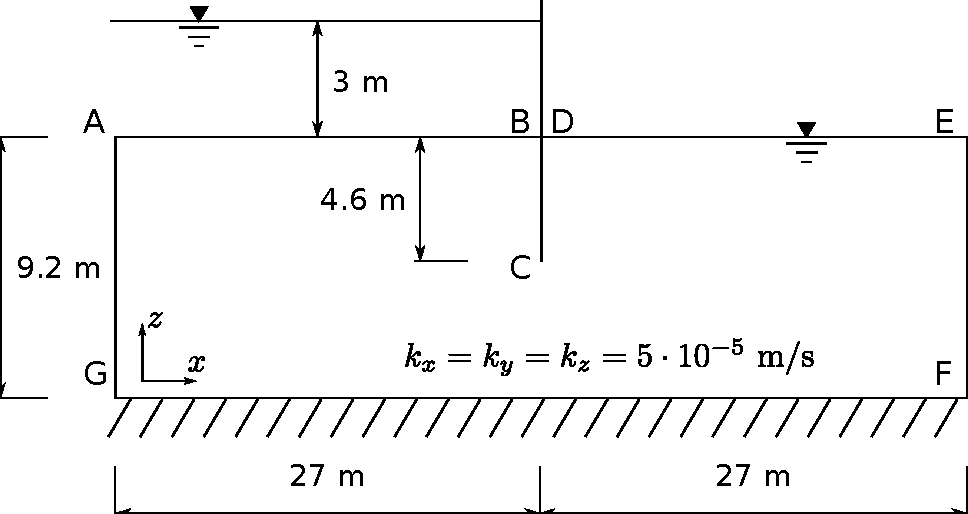
\includegraphics[width=0.75\textwidth]{./body/images/enu01}
  \end{center}
  \caption{Descripción del modelo}
  \label{enu01}
\end{figure}

Las unidades que vamos a utilizar se resumen en el Cuadro \ref{tab:201}:
\begin{table}[!h]
  \centering
  \begin{tabular}{lc}
\hline
Magnitud&Unidades\\
\hline
  Longitud & m\\
  Altura total del fluido $h$ & m \\
  Coeficiente permeabilidad $k$ & m/s\\
  Vector flujo $\mathbf{q}$ & m$^3$/s/m$^2$ \\
  Gradiente hidraúlico $\mathbf{i}_h$ & m/m \\
\hline
  \end{tabular}
  \caption{Unidades del problema}
  \label{tab:201}
\end{table}

Para resolver este problema iniciamos Abaqus como en la práctica del tema 1 y 
definimos un directorio de trabajo llamado \textit{Practica02}. A continuación
se describen las acciones a realizar en cada uno de los módulos para llevar
a cabo el análisis. 

\subsection{Módulo Part. Crear la geometría de los elementos}
Activamos el módulo \textit{Part} (ver Fig.~\ref{part01}) y creamos un
nuevo objeto tipo \textbf{2D Planar}, \textbf{Deformable} y
\textbf{Shell} (ver Fig.~\ref{part02}).

  \begin{figure}
    \centering
    \begin{subfigure}[!h]{0.29\textwidth}
      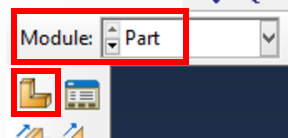
\includegraphics[width=\textwidth]{./body/images/part01.pdf}
      \caption{Inicio módulo \textbf{Part}}
      \label{part01}
    \end{subfigure}%
    ~ %add desired spacing between images, e. g. ~, \quad, \qquad, \hfill etc.
    % (or a blank line to force the subfigure onto a new line)
    \begin{subfigure}[!h]{0.39\textwidth}
      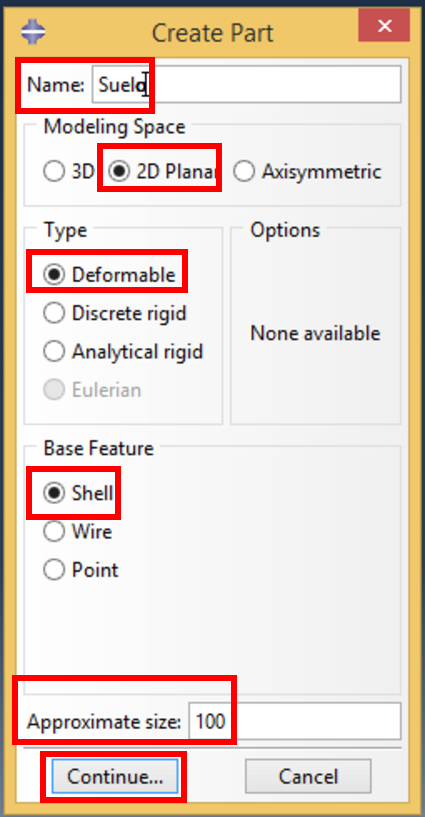
\includegraphics[width=\textwidth]{./body/images/part02.pdf}
      \caption{cuadro de diálogo \textbf{Create Part}}
      \label{part02}
    \end{subfigure}%
    \caption{Inicio módulo \textbf{Part} y cuadro de diálogo
      \textbf{Create Part}}
  \end{figure}
  Con la herramienta \textit{Sketcher} definimos la geometría del
  problema como indica la Fig.~\ref{part03} obteniendo finalmente la nueva
  \textit{part} que muestra la Fig.~\ref{part04}.
  \begin{figure}
    \centering
    \begin{subfigure}[!h]{1.0\textwidth}
      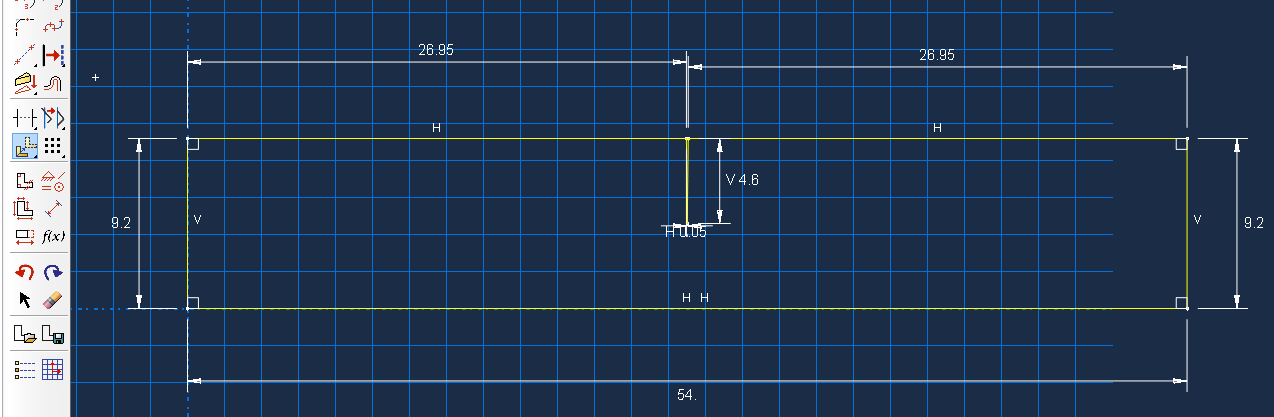
\includegraphics[width=\textwidth]{./body/images/part03}
      \caption{Definición de la geometría}
      \label{part03}
    \end{subfigure}%
    
  %add desired spacing between images, e. g. ~, \quad, \qquad, \hfill etc.
    % (or a blank line to force the subfigure onto a new line)
    \begin{subfigure}[!h]{0.875\textwidth}
      
\includegraphics[width=\textwidth]{./body/images/part04}
      \caption{Nueva \textbf{Part}}
      \label{part04}
    \end{subfigure}%
    \caption{Construcción de una nueva \textbf{Part}}
  \end{figure}

  \subsection{Modulo Property. Definir materiales y secciones}

  Acitvamos ahora el módulo \textbf{Property} y definimos un nuevo
  material tipo \textbf{Thermal}, \textbf{Isotropic} y con una
  conductividad de $5\cdot 10^{-5}$ tal como muestras las
  Figs.\ref{prop01} a \ref{prop03}.
  \begin{figure}
    \centering
    \begin{subfigure}[!h]{0.22\textwidth}
      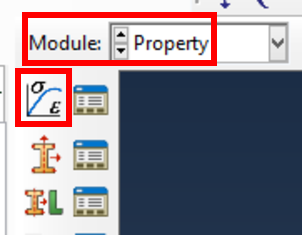
\includegraphics[width=\textwidth]{./body/images/prop01.pdf}
      \caption{Comando \textbf{Create Material}}
      \label{prop01}
    \end{subfigure}%
    ~ %add desired spacing between images, e. g. ~, \quad, \qquad, \hfill etc.
    % (or a blank line to force the subfigure onto a new line)
    \begin{subfigure}[!h]{0.36\textwidth}
      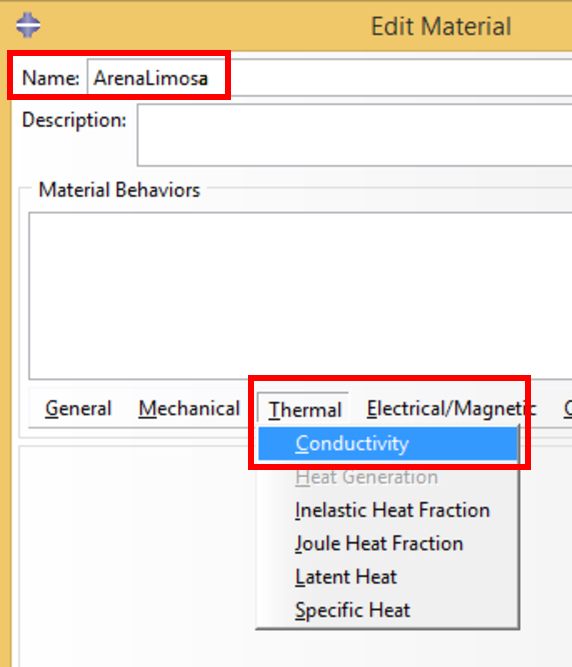
\includegraphics[width=\textwidth]{./body/images/prop02.pdf}
      \caption{Selección tipo de comportamiento}
      \label{prop02}
    \end{subfigure}%
    ~
    \begin{subfigure}[!h]{0.36\textwidth}
      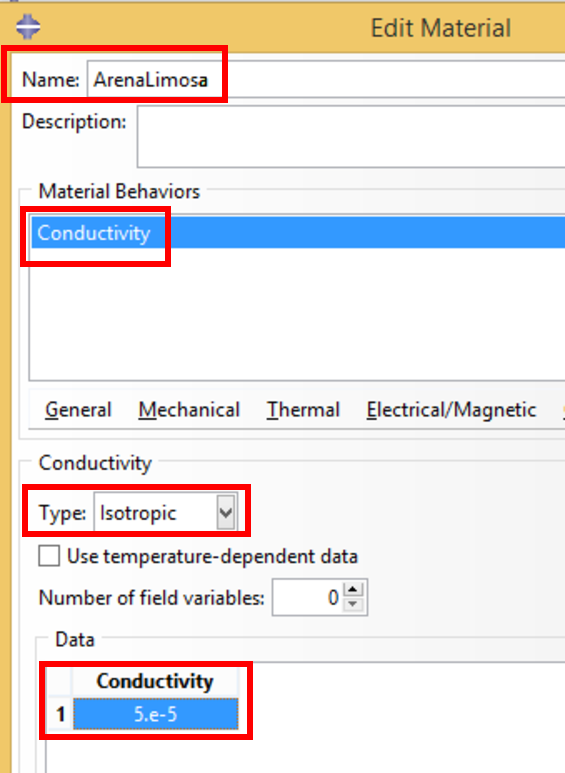
\includegraphics[width=\textwidth]{./body/images/prop03.pdf}
      \caption{Definición parámetros del material}
      \label{prop03}
    \end{subfigure}%
    \caption{Definición de un nuevo material}
  \end{figure}

  Una vez definido el material debemos definir una nueva sección de
  tipo \textbf{Solid} y \textbf{Homogeneous} siguiendo los pasos de
  las Figs.~\ref{prop03p} a \ref{prop05}.

  \begin{figure}
    \centering
    \begin{subfigure}[!h]{0.20\textwidth}
      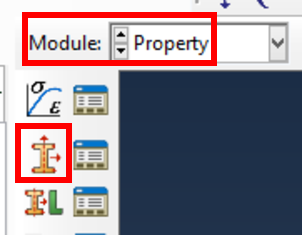
\includegraphics[width=\textwidth]{./body/images/prop03p.pdf}
      \caption{Comando \textbf{Create Section}}
      \label{prop03p}
    \end{subfigure}%
    ~
    \begin{subfigure}[!h]{0.39\textwidth}
      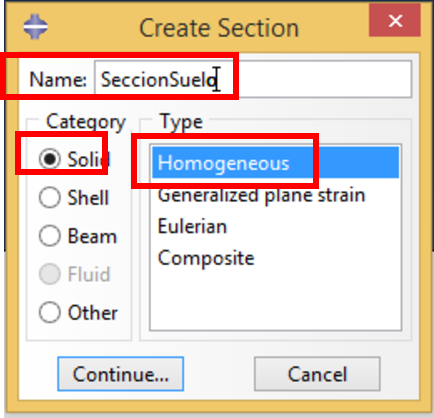
\includegraphics[width=\textwidth]{./body/images/prop04.pdf}
      \caption{Definición propiedades de la sección}
      \label{prop04}
    \end{subfigure}%
    ~ %add desired spacing between images, e. g. ~, \quad, \qquad, \hfill etc.
    % (or a blank line to force the subfigure onto a new line)
    \begin{subfigure}[!h]{0.39\textwidth}
      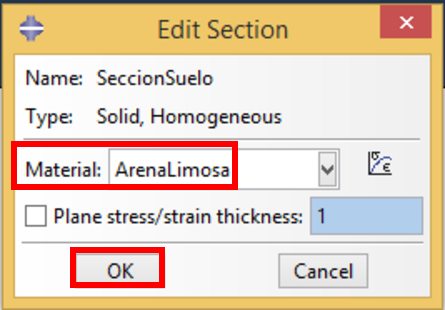
\includegraphics[width=\textwidth]{./body/images/prop05.pdf}
      \caption{Asignación del material a la sección}
      \label{prop05}
    \end{subfigure}%
    \caption{Definición de la sección \textit{SeccionSuelo}}
  \end{figure}

  Finalmente asignamos la sección creada a la \textbf{part} según se
  resume en las Figs.~\ref{prop05p} a \ref{prop07}.

  \begin{figure}
    \centering
    \begin{subfigure}[!h]{0.20\textwidth}
      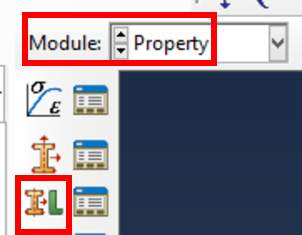
\includegraphics[width=\textwidth]{./body/images/prop05p.pdf}
      \caption{Comando \textbf{Assign Section}}
      \label{prop05p}
    \end{subfigure}%
    ~
    \begin{subfigure}[!h]{0.39\textwidth}
      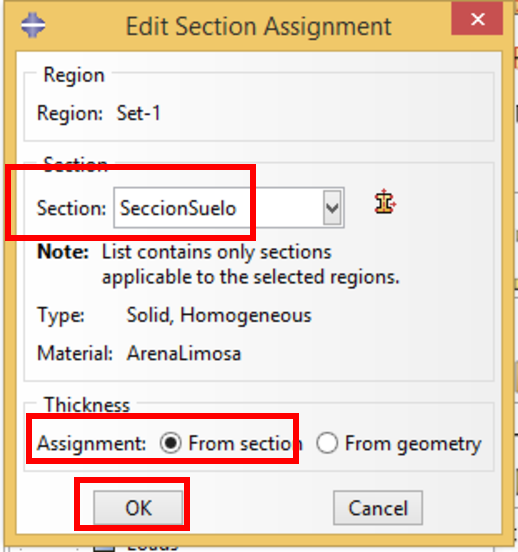
\includegraphics[width=\textwidth]{./body/images/prop06.pdf}
      \caption{Vinculación sección a \textit{Part}}
      \label{prop06}
    \end{subfigure}%
    
    % add desired spacing between images, e. g. ~, \quad, \qquad,
    % \hfill etc.
    % (or a blank line to force the subfigure onto a new line)
    \begin{subfigure}[!h]{0.75\textwidth}
      
\includegraphics[width=\textwidth]{./body/images/prop07.png}
      \caption{\textit{Part} con sección asignada}
      \label{prop07}
    \end{subfigure}%
    \caption{Asignación de la sección a una \textbf{Part}}
  \end{figure}

  \subsection{Módulo Assembly. Ensamblar el modelo}

  En el módulo \textit{Assembly} ensamblamos nuestro modelo haciendo
  una copia \textbf{dependiente} de nuestra \textit{part} tal como
  indican las Figs.~\ref{asse01} y \ref{asse02}.

  \begin{figure}
    \centering
    \begin{subfigure}[!h]{0.25\textwidth}
      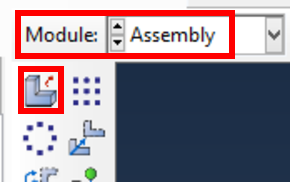
\includegraphics[width=\textwidth]{./body/images/asse01.pdf}
      \caption{Comando \textbf{Create Instance}}
      \label{asse01}
    \end{subfigure}%
    ~ %add desired spacing between images, e. g. ~, \quad, \qquad, \hfill etc.
    % (or a blank line to force the subfigure onto a new line)
    \begin{subfigure}[!h]{0.39\textwidth}
      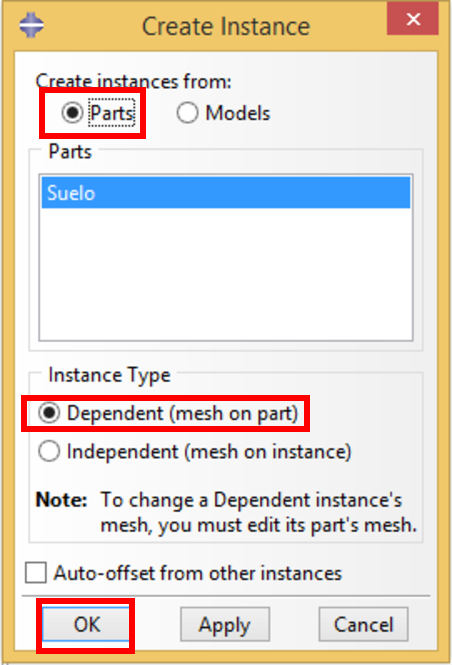
\includegraphics[width=\textwidth]{./body/images/asse02.pdf}
      \caption{Creacción de una copia \textbf{Dependiente}}
      \label{asse02}
    \end{subfigure}%
    \caption{Acción \textbf{Create Instance}}
  \end{figure}

  \subsection{Módulo Step. Configurar el procedimiento de análisis}

  Necesitamos crear un caso de cálculo de tipo \textbf{Heat Transfer}
  indicándo que va a ser \textbf{estacionario} (\textbf{Steady-state})
  (ver Figs.~\ref{step01} a \ref{step03}).


  \begin{figure}
    \centering
    \begin{subfigure}[!h]{0.20\textwidth}
      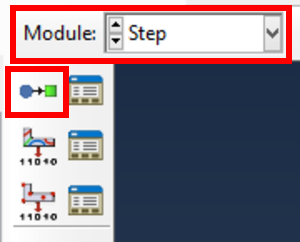
\includegraphics[width=\textwidth]{./body/images/step01.pdf}
      \caption{Comando \textbf{Create Step}}
      \label{step01}
    \end{subfigure}%
    ~
    \begin{subfigure}[!h]{0.39\textwidth}
      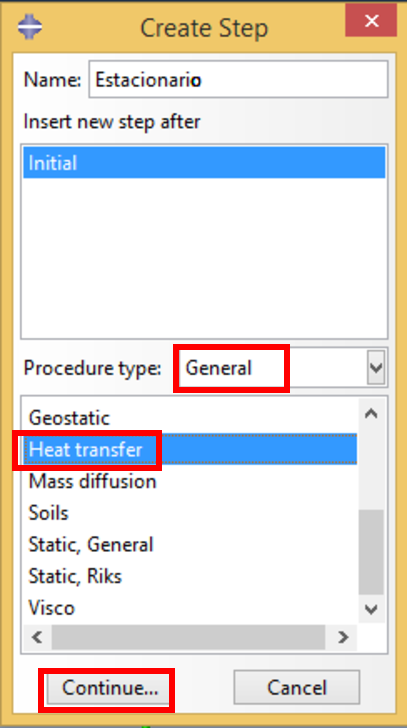
\includegraphics[width=\textwidth]{./body/images/step02.pdf}
      \caption{Propiedades nuevo caso de cálculo}
      \label{step02}
    \end{subfigure}%
    ~ %add desired spacing between images, e. g. ~, \quad, \qquad, \hfill etc.
    % (or a blank line to force the subfigure onto a new line)
    \begin{subfigure}[!h]{0.39\textwidth}
      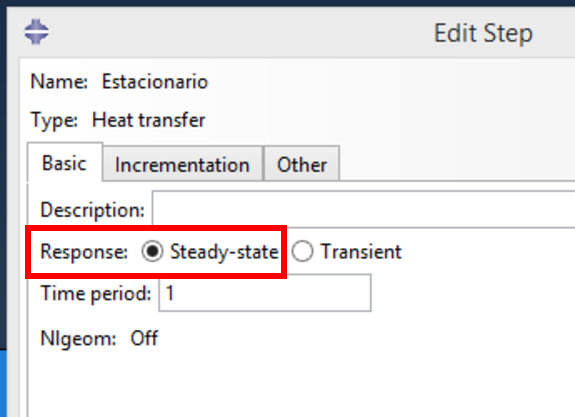
\includegraphics[width=\textwidth]{./body/images/step03.pdf}
      \caption{Selección análisis estacionario}
      \label{step03}
    \end{subfigure}%
    \caption{Creación de un nuevo caso de cálculo}
  \end{figure}

  Al haber haber definido un régimen estacionario Abaqus no nos
  genera un \textbf{History Output}. Revisemos entonces los datos que
  le vamos a pedir que nos guarde para el postproceso abriendo el
  \textbf{Field Output} que crea por defecto, y asegurándonos que
  guardamos las \textbf{temperaturas nodales}, el \textbf{vector de
    flujo de calor} y los \textbf{flujos de reacción} (allí donde
  aplicamos una condición de contorno tipo Dirchlet de temperatura)
  tal como indican las Figs.~\ref{step04} y \ref{step05}.

  \begin{figure}
    \centering
    \begin{subfigure}[!h]{0.45\textwidth}
      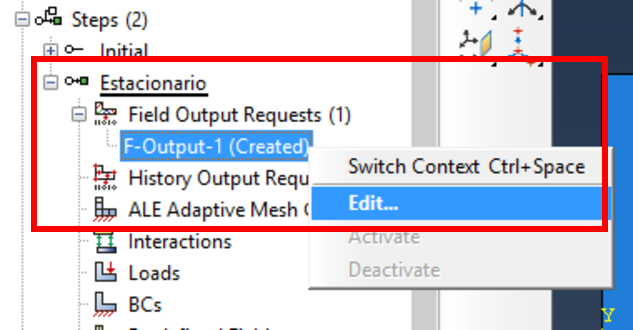
\includegraphics[width=\textwidth]{./body/images/step04.pdf}
      \caption{Selección del \textbf{Field Output}}
      \label{step04}
    \end{subfigure}%
    ~ %add desired spacing between images, e. g. ~, \quad, \qquad, \hfill etc.
    % (or a blank line to force the subfigure onto a new line)
    \begin{subfigure}[!h]{0.45\textwidth}
      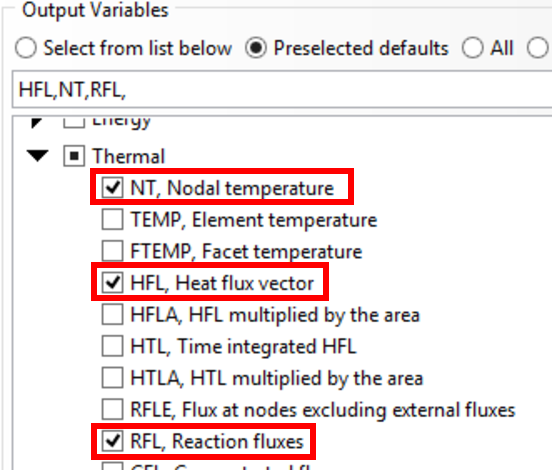
\includegraphics[width=\textwidth]{./body/images/step05.pdf}
      \caption{Valores a guardar para el postproceso}
      \label{step05}
    \end{subfigure}%
    \caption{Definición del \textit{Field Output}}
  \end{figure}

  \subsection{Módulo Load. Aplicar las condiciones de contorno}

  En el caso de problemas de flujo confinados podemos encontrar las
  siguientes dos condiciones de contorno (en nuestro problema
  impondremos un valor constante a las condiciones de contorno porque
  asumimos estamos en un régimen estacionario) :
  \begin{description}
  \item[Tipo Dirichlet] Contornos donde imponemos el valor de la carga
    total del fluido $h=h^*$.
  \item[Tipo Neumann] Contorno donde imponemos el valor del flujo
    $(-\textbf{k}\cdot\bm{\nabla}h)\cdot\textbf{n}=\mathrm{cte}$,
    siendo $\textbf{n}$ la normal exterior al contorno donde imponemos
    el valor del flujo.
  \end{description}

  Si no imponemos nada en un contorno de nuestro dominio, Abaqus
  entiende que estamos imponiendo que el flujo a través de esa
  frontera es nulo (frontera impermeable), lo que se traduce que
  estamos imponiendo $ \bm{\nabla}h\cdot\textbf{n}=0$.

  En nuestro caso tenemos que imponer:
  \begin{enumerate}
  \item Dos condiciones de contorno tipo Dirichlet en la parte
    superior del dominio (asumiendo que el datum está en la línea
    horizontal AE)
    \begin{itemize}
    \item $h=u_A/\gamma_w+z_A=\dfrac{\rho_w\; g\; 3}{\rho_w g}+0 = 3$
      m en la equipotencial AB
    \item $h=u_E/\gamma_w+z_E= \dfrac{\rho_w\; g\; 0}{\rho_w g}+0=0$ m
      en la equipotencial DE
    \end{itemize}
    Estas condiciones las impondremos en el caso de carga creado he
    hemos llamado \textit{estacionario}.
  \item La condición de contorno tipo Neuman de frontera impermeable $
    \bm{\nabla}h\cdot\textbf{n}=0$ en los contornos AGFE y BCD. Esta
    condición de contorno se mantiene fija en todo el análisis y la
    podríamos definir en el caso de carga creado por Abaqus
    \textit{Initial} para que se propage al resto de casos de
    carga. Sin embargo, como esta condición (frontera impermeable) se
    define por defecto, no es necesario que definamos nada.
  \end{enumerate}

  Para imponer la condición de contorno tipo Dirichlet $h=3$ en el
  contorno AB activamos el módulo \textbf{Load} y pulsamos la orden
  \textbf{Create Boundary Condition} (ver Fig.~\ref{load02}). Después
  sigue las instrucciones indicadas en las Figs.~\ref{load03} a
  \ref{load05}.

  \begin{figure}
    \centering
    \begin{subfigure}[!h]{0.25\textwidth}
      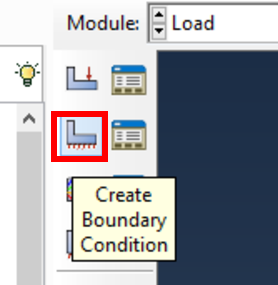
\includegraphics[width=\textwidth]{./body/images/load02.pdf}
      \caption{Comando \textbf{Create Boundary Condition}}
      \label{load02}
    \end{subfigure}%
    ~ %add desired spacing between images, e. g. ~, \quad, \qquad, \hfill etc.
    % (or a blank line to force the subfigure onto a new line)
    \begin{subfigure}[!h]{0.45\textwidth}
      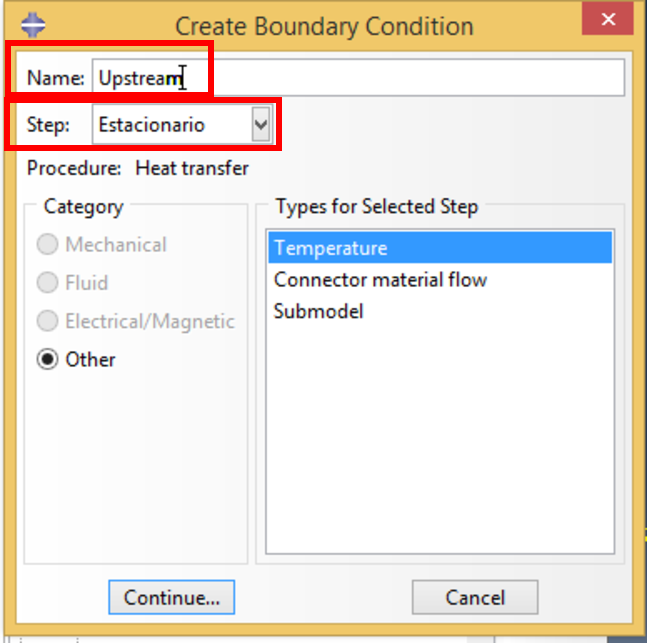
\includegraphics[width=\textwidth]{./body/images/load03.pdf}
      \caption{Definición tipo de condición Dirichlet}
      \label{load03}
    \end{subfigure}%

    \begin{subfigure}[!h]{0.52\textwidth}
      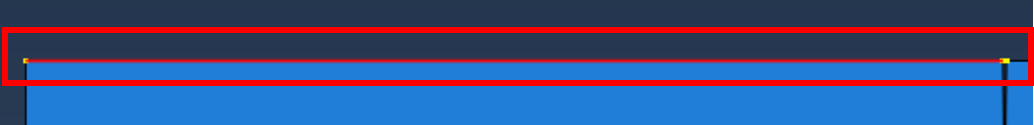
\includegraphics[width=\textwidth]{./body/images/load04.pdf}
      \caption{Selección de la frontera}
      \label{load04}
    \end{subfigure}%
    ~ %add desired spacing between images, e. g. ~, \quad, \qquad, \hfill etc.
    % (or a blank line to force the subfigure onto a new line)
    \begin{subfigure}[!h]{0.45\textwidth}
      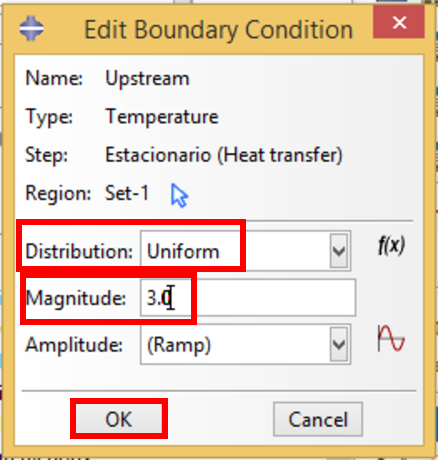
\includegraphics[width=\textwidth]{./body/images/load05.pdf}
      \caption{Definición de la altura total impuesta}
      \label{load05}
    \end{subfigure}%
    \caption{Definición de la condición de contorno en la
      equipotencial AB}
  \end{figure}

  De igual manera, para imponer las condición de contorno tipo
  Dirichlet $h=0$ en el contorno DE sigue las instrucciones indicadas
  en las Figs.~\ref{load06} a \ref{load08}. Al final Abaqus indica las
  fronteras donde has impuesto las condiciones de contorno tal como
  muestra la Fig.~\ref{load09}.

  \begin{figure}
    \centering
    \begin{subfigure}[!h]{0.42\textwidth}
      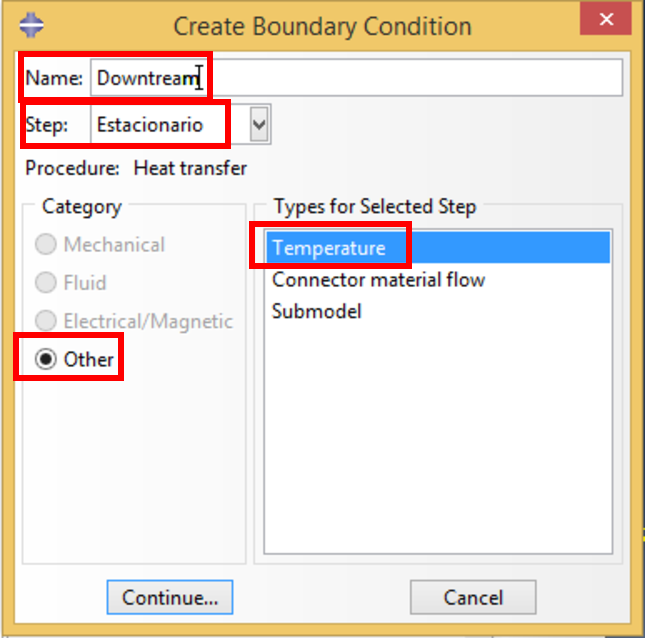
\includegraphics[width=\textwidth]{./body/images/load06.pdf}
      \caption{Definición tipo de condición Dirichlet}
      \label{load06}
    \end{subfigure}%
    ~ %add desired spacing between images, e. g. ~, \quad, \qquad, \hfill etc.
    % (or a blank line to force the subfigure onto a new line)
    \begin{subfigure}[!h]{0.55\textwidth}
      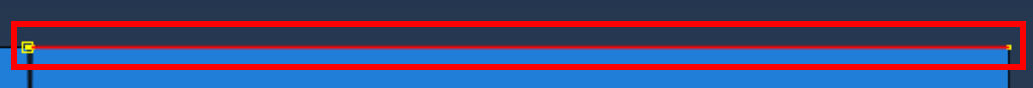
\includegraphics[width=\textwidth]{./body/images/load07.pdf}
      \caption{Selección de la frontera}
      \label{load07}
    \end{subfigure}%

    \begin{subfigure}[!h]{0.42\textwidth}
      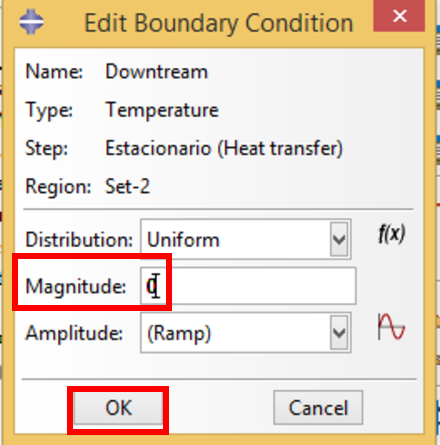
\includegraphics[width=\textwidth]{./body/images/load08.pdf}
      \caption{Definición de la altura total impuesta}
      \label{load08}
    \end{subfigure}%
    ~ %add desired spacing between images, e. g. ~, \quad, \qquad, \hfill etc.
    % (or a blank line to force the subfigure onto a new line)
    \begin{subfigure}[!h]{0.55\textwidth}
      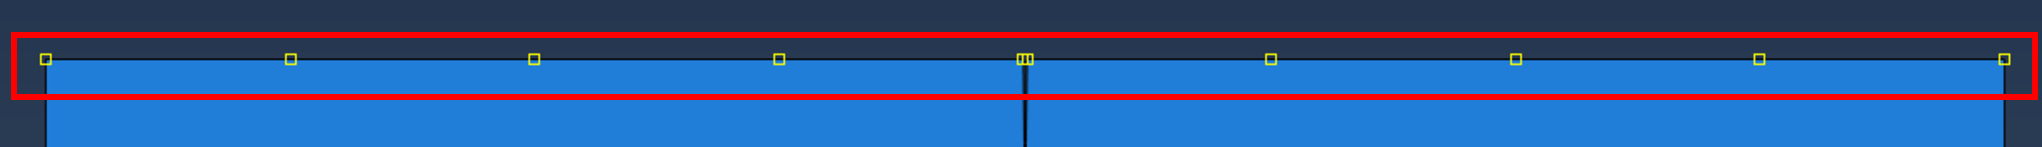
\includegraphics[width=\textwidth]{./body/images/load09.pdf}
      \caption{Indicación fronteras con condiciones impuestas}
      \label{load09}
    \end{subfigure}%
    \caption{Definición de la condición de contorno en la
      equipotencial DE}
  \end{figure}


\subsection{Módulo Mesh. Crear la malla.}

Para construir la malla recordamos los pasos a siguir tal como se
indicaron en la práctica 1:
\begin{enumerate}
\item Activo el módulo \textbf{Mesh} y, dado que hemos ensamblado el modelo con una copia dependiente, impongo que voy a mallar la \textbf{part} tal como indica la Fig.%\ref
  \begin{figure}[!h]
    \begin{center}
      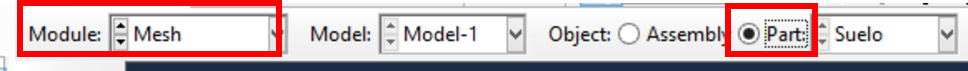
\includegraphics[width=0.9\textwidth]{./body/images/mess01.pdf}
    \end{center}
    \caption{Inicio del módulo \textbf{mesh}}
 \label{mess01}
  \end{figure}

\item Defino la forma del elemento (serán cuadriláteros) (ver Fig.~\ref)
\item Defino el tamaño global del elemento a 1.5 metros (ver Fig.~\ref)
\item Finalmente defino el tipo de interpolación tal como indica la Fig.\ref
\end{enumerate}
  \hspace{20mm}\hrulefill$\star$\hrulefill\hspace{20mm}
